%%%%%%%%%%%%%%%%%%%%%%%%%%%%%%%%%%%%%%%%%%%%%%%%%%%%%%%%%%%%%%%%%%%%%%%%%%%%%%%%
%% Projeto Final de Graduação
%% Aluno: Victor Seixas Souza
%% Orientadora: Christiane Neme Campos
%% Tema: Teoria de Ramsey em Grafos
%%%%%%%%%%%%%%%%%%%%%%%%%%%%%%%%%%%%%%%%%%%%%%%%%%%%%%%%%%%%%%%%%%%%%%%%%%%%%%%%
% !TEX root = ../thesis.tex
%%%%%%%%%%%%%%%%%%%%%%%%%%%%%%%%%%%%%%%%%%%%%%%%%%%%%%%%%%%%%%%%%%%%%%%%%%%%%%%%

\chapter{Introdução}

No primeiro dia de aula em uma escolinha de matemática, a professora preparou uma gincana para entrosar os alunos. Ela os sorteou em grupos de seis, e cada grupo deveria sentar-se em mesas separadas. O objetivo era que os alunos conversasem entre si sobre o que fizeram durante as férias e, potencialmente, criassem novas amizades. Alguns alunos haviam sido colegas nos anos anteriores e, portanto, já se conheciam; outros alunos vieram de turmas diferentes, então não conheciam a todos. Além disso, novos alunos entram na escola todo ano para aprender matemática!

Após o sorteio, a professora supervisionou atentamente os grupos e observou que em algumas mesas, três alunos já se conheciam. Já em outras mesas, até quatro alunos já se conheciam. Preocupada se a gincana teria o efeito desejado, ela adotou outra estratégia e focou apenas nos alunos que ainda não se conheciam. Em algumas mesas, havia três alunos que ainda não se conheciam, mas outras pareciam menos promissoras, não havendo nem três alunos que não se conheciam. O fato curioso era que nestas mesas haviam três alunos que se conheciam. Sendo uma professora de matemática, ela se perguntou se existia algum motivo para isto acontecer. Será que se ela fizesse outro sorteio, poderia haver uma mesa em que nenhum grupo de três alunos se conhecessem e nenhum grupo de três alunos não se conhecessem? Por sorte, a professora havia estudado Teoria de Grafos, e conseguiu verificar o seguinte fato:

%%%%%%%%%%%%%%%%%%%%%%%%%%%%%%%%%%%%%%%%
\begin{fact} \label{fact:intro:ramsey}
Em uma mesa com seis alunos, três alunos se conhecem ou três alunos não se conhecem.
\end{fact}
%%%%%%%%%%%%%%%%%%%%%%%%%%%%%%%%%%%%%%%%

Vamos ver agora como que a professora percebeu este fato. Considere que você seja um dos seis alunos da mesa. Dos cinco restantes, você conhece uma quantidade, digamos $c$, e também não conhece uma quantidade $n$. Sabemos que $c + n = 5$. Isto nos dá que, ou $c \geq 3$, ou $n \geq 3$. De fato, se $c \leq 2$ e $n \leq 2$ occorrerem simultaneamente, $5 = c + n \leq 4$, o que é absurdo. Suponha $c \geq 3$, isto significa que você conhece pelo menos três dos outros alunos, digamos Alberto, Bruna e Carlos. Se existe alguma amizade entre eles, digamos, Alberto e Carlos são amigos, então a mesa possui um grupo de três alunos que se conhece, você, Alberto e Carlos. Caso isto não ocorra, então Alberto, Bruna e Carlos formam um grupo de três alunos que não se conhecem. O caso $n \geq 3$ segue do mesmo raciocínio.

O Fato \ref{fact:intro:ramsey} pode ser considerado o primeiro resultado na Teoria de Ramsey e possui generalizações interessantes. Além disso, ele possui uma formulação mais clara em termos de coloração de grafos. Na próxima seção, introduzimos os conceitos da Teoria de Grafos que são necessários para adentrar o universo da Teoria de Ramsey em grafos. Um leitor familiarizado com grafos é convidado a fazer uma leitura rápida da seção para se familiarizar à notação utilizada neste texto.

%%%%%%%%%%%%%%%%%%%%%%%%%%%%%%%%%%%%%%%%%%%%%%%%%%%%%%%%%%%%%%%%%%%%%%%%%%%%%%%%

\section{Noções de Grafos}

Um \indef{grafo} $G$ é um par ordenado $(V(G), E(G))$, que consiste em um conjunto $V(G)$ de \indef{vértices} e um conjunto $E(G)$ de \indef{arestas}, disjunto de $V(G)$, em conjunto com uma função de incidência $\Psi_G$ que associa cada aresta de $G$ a um par de vértices de $G$, não necessariamente distintos.
Uma aresta $e \in E(G)$ e vértices $u, v \in V(G)$ são ditos \indef{incidentes} se $\Psi_G(e) = \{u,v\}$. Neste caso, diz-se ainda que $u$ e $v$ são as \indef{extremidades} de $e$. A incidência relaciona elementos de conjuntos distintos, neste caso, vértices e arestas.
Uma outra relação é a de adjacência, que se aplica para elementos de mesma natureza. Dois vértices $u$ e $v$ são ditos \indef{adjacentes} em $G$ se existe uma aresta $e$ em $G$ tal que $\Psi_G(e) = \{u,v\}$. Duas arestas $e$ e $f$ são ditas \indef{adjacentes} em $G$ se existe um vértice $v$ em $G$ tal que $v \in \Psi_G(e) \cap \Psi_G(f)$, isto é, se existe um vértice $v$ que incide simultaneamente em $e$ e $f$.

Vamos construir um grafo $G = (V(G), E(G))$ para ilustrar estas definições. O conjunto de vértices será $V(G) = \{u,v,w,x\}$ e o conjunto de arestas será $E(G) = \{e, f, g, h, j, k, l, s\}$. Falta definir a função de incidência $\Psi_G$, que associa as arestas aos vértices:
\begin{align*}
\Psi_G(e) = \{v,x\} & &
\Psi_G(f) = \{u,v\} & &
\Psi_G(g) = \{u,v\} & &
\Psi_G(h) = \{v,w\} \\
\Psi_G(j) = \{v,w\} & &
\Psi_G(k) = \{u,x\} & &
\Psi_G(l) = \{w,x\} & &
\Psi_G(s) = \{x\}
\end{align*}

Isto completa a definição do grafo $G$. Uma maneira interessante de representar grafos é por meio de um desenho. A Figura \ref{fig:intro:grafo} representa o grafo $G$ da seguinte maneira: os vértices são indicados por círculos e as arestas são indicadas por linhas que unem os círculos que correspondem aos vértices nos quais a aresta incide. A representação gráfica é muito importante pois nos permite criar uma intuição sobre a estrutura de grafos. Vale a pena notar que um mesmo grafo pode possuir mais de um desenho: basta desenhar os vértices em posições diferentes do plano. De fato, a posição dos vértices e das arestas não é importante, é a relação entre os vértices e as arestas que caracteriza a estrutura do grafo.

%%%%%%%%%%%%%%%%%%%%%%%%%%%%%%%%%%%%%%%%
\begin{figure}[ht!]
\centering
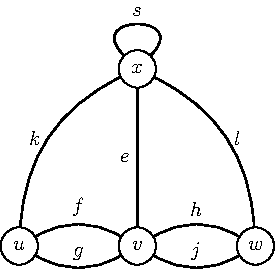
\includegraphics{figures/1_intro_1_grafo}
\caption{Representação gráfica do grafo $G$.}
\label{fig:intro:grafo}
\end{figure}
%%%%%%%%%%%%%%%%%%%%%%%%%%%%%%%%%%%%%%%%

O desenho de um grafo pode ser um bom representante da estrutura, mas dois grafos com o mesmo desenho não são necessariamente iguais. Do ponto de vista formal, dois grafos $G$ e $H$ são idênticos quando $G = H$ no sentido da Teoria de Conjuntos, isto é, $V(G)$ e $V(H)$ são o mesmo conjunto, $E(G)$ e $E(H)$ são o mesmo conjunto e $\Psi_G$ e $\Psi_H$ são a mesma função. Por exemplo, os grafos $G$ e $H$ da Figura \ref{fig:intro:iso} não são idênticos pois $V(G) \neq V(H)$, no entanto, eles possuem efetivamente a mesma estrutura.

Esta noção de igualdade de grafos é, como vimos, muito restritiva. Para capturar a noção de que dois grafos diferentes podem ter a mesma estrutura, definimos um \indef{isomorfismo} entre dois grafos $G$ e $H$ como um par de bijeções $\theta : V(G) \to V(H)$ e $\phi : E(G) \to E(G)$ tais que elas preservam a relação de incidência, isto é, $\Psi_G(e) = \{u,v\}$ se e somente se $\Psi_H(\phi(e)) = \{\theta(u),\theta(v)\}$. Quando existe um isomorfismo entre dois grafos $G$ e $H$, dizemos que eles são \indef{isomorfos}, e escrevemos $G \iso H$.

%%%%%%%%%%%%%%%%%%%%%%%%%%%%%%%%%%%%%%%%
\begin{figure}[ht!]
\centering
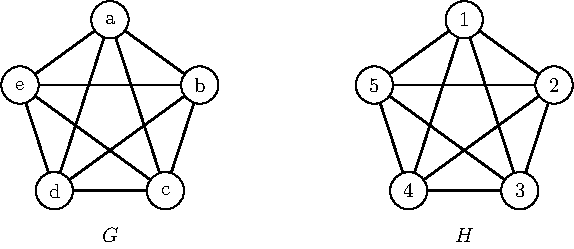
\includegraphics{figures/1_intro_2_iso}
\caption{Dois grafos não idênticos $G$ e $H$ que são isomorfos.}
\label{fig:intro:iso}
\end{figure}
%%%%%%%%%%%%%%%%%%%%%%%%%%%%%%%%%%%%%%%%

Grafos isomorfos possuem essencialmente a mesma estrutura e são considerados como iguais para todos os efeitos práticos. Com efeito, muitas vezes, os nomes que os vértices possuem não tem nenhuma importância. Quando abrimos mão de definir os nomes dos vértices, temos um \indef{grafo não rotulado}, em contrapartida com os \indef{grafos rotulados}. Muitas vezes, apenas nos interessa a interconectividade dos vértices, então consideramos grafos não rotulados e nomeamos os vértices e arestas conforme necessário.

Formalmente, a relação de isomorfismo $\iso$ é uma relação de equivalência na classe de todos os grafos. As classes de equivalência são compostas por grafos rotulados que são equivalentes sob a relação de isomorfismo. Grafo não rotulado é um nome que damos a uma destas classes de equivalência, não sendo um grafo propriamente dito, e sim uma entidade abstrata que carrega em si a estrutura de um grafo sem incluir os rótulos dos vértices e das arestas.

O que nos permite escolher um representante dentro desta classe sem perda de generalidade é o fato de que a maioria das propriedades estudadas pela Teoria de Grafos é invariante por isomorfismo, isto é, se um grafo tem determinada propriedade, qualquer grafo isomorfo a ele possui a mesma propriedade. Portanto, ao rotular vértices e arestas de um grafo não rotulado, podemos fazer o mesmo de forma arbitrária e sem perda de generalidade.

Uma outra noção fundamental é a de \indef{subgrafo}. Seja $G$ um grafo, dizemos que $H$ é um subgrafo de $G$ se $H$ for um grafo tal que $V(H) \subset V(G)$, $E(H) \subset E(G)$ e $\Psi_H$ é restrição de $\Psi_G$. Quando $H$ é subgrafo de $G$, também dizemos que $G$ possui $H$, ou que existe uma cópia de $H$ em $G$. Em geral, diremos que $H$ é um subgrafo de $G$ quando existir subgrafo de $G$ isomorfo a $H$.

Uma noção ligeiramente distinta de subgrafo é a de \indef{subgrafo induzido}. Seja $G = (V,E)$ um grafo e $S \subset V$ um subconjunto de vértices. O grafo $G[S]$ é o grafo cujo conjunto de vértices é $S$ e cujo conjunto de arestas consiste nas arestas de $G$ que possuem ambas extremidades em $S$. Dizemos que $G[S]$ é um subgrafo de $G$ \indef{induzido} pelo conjunto $S$.

Até agora, a definição de grafos que temos é bastante abrangente e permite algumas situações que não gostaríamos de considerar em nosso estudo. A primeira situação especial ocorre quando duas arestas $e$ e $f$ incidem nos mesmos vértices, isto é, $\Psi_G(e) = \Psi_G(f)$, neste caso dizemos que $e$ e $f$ são \indef{arestas paralelas}. No grafo exemplificado na Figura \ref{fig:intro:grafo}, $f$ e $g$ são arestas paralelas.
A segunda situação é quando $e$ incide em apenas um vértice $v$, isto é, $\Psi_G(e) = \{v\}$, como é o caso da aresta $s$ da Figura \ref{fig:intro:grafo}, e dizemos que esta aresta é um \indef{laço}. Um grafo no qual não existem arestas paralelas ou laços é dito um \indef{grafo simples}. Neste estudo, consideraremos apenas grafos simples.

Seja $G$ um grafo simples e $u$ e $v$ dois vértices de $G$. Se $u$ e $v$ forem adjacentes, então existe uma única aresta $e$ em $G$ com $\Psi_G(e) = \{u,v\}$, portanto podemos identificar $e$ por $\{u,v\}$. De fato, quando $G$ é simples, a função de incidência $\Psi_G$ fica definida implicitamente e nomeamos as arestas por suas extremidades. Portanto, ao definir grafos simples, pode-se omitir a função de incidência $\Psi$ definindo o conjunto das arestas $E(G)$ como um subconjunto de pares de vértices. Para tal propósito, para um conjunto $S$, definimos o conjunto de pares de elementos de $S$ por $S^{(2)}$, assim, podemos ver um grafo como um par $G = (V(G),E(G))$ no qual $E(G) \subset V(G)^{(2)}$.

Para simplificar a notação, quando não houver ambiguidade, podemos nos referir ao conjunto de vértices apenas por $V$ e o conjunto de arestas por $E$ em um grafo $G = (V,E)$. A quantidade de vértices de um grafo é chamada de \indef{ordem} do grafo e costuma ser denotada por $n$ ou $v(G)$. Já a quantidade de arestas em um grafo é chamada de \indef{tamanho} do grafo, e é denotada por $m$ ou $e(G)$. Se $G$ é um grafo simples, observamos que $E \subset V^{(2)}$, o que implica que $m \leq \binom{n}{2} = O(n^2)$, isto é, um grafo simples tem uma quantidade de arestas limitada ao quadrado do seu número de vértices.

Se $v$ é um vértice de um grafo $G$ simples, então a \indef{vizinhança} $N_G(v)$ de $v$ é o conjunto dos vértices adjacentes a $v$. O \indef{grau} de um vértice $d_G(v)$ é a cardinalidade de sua vizinhança\footnote{Esta definição de grau de um vértice está restrita a grafos simples. No caso geral, um grau de um vértice $v$ é a quantidade de vezes que arestas incidem nele, isto é, o o número de arestas que incidem em $v$ com os laços contados duas vezes.}, isto é, $d_G(v) = \card{N_G(v)}$. Quando o grafo for conhecido pelo contexto, utilizamos apenas $N(v)$ e $d(G)$.

Seja $G = (V,E)$ um grafo simples, vamos contar o número de arestas de duas maneiras distintas. Cada vértice $v$ incide em $d(v)$ arestas, portanto, consideramos a soma $\sum_{v \in V}d(v)$ as arestas de $G$. No entanto, cada aresta incide em exatamente dois vértices, já que o grafo é simples. Isto nos dá que a soma conta todas as arestas exatamente duas vezes, logo $\sum_{v \in V}d(v) = 2|E|$. Este resultado é conhecido por \emph{handshaking lemma}, e é demasiadamente útil. Uma primeira aplicação é a observação de que um grafo simples só pode ter uma quantidade par de vértices de grau ímpar. De fato, o resultado anterior nos dá que a soma dos graus dos vértices de $G$ é sempre par, e se $A$ é o conjunto de vértices de grau ímpar, temos $\sum_{v \in V}d(v) \equiv |A| \equiv 0 \Mod{2}$.

Algumas vezes, grafos que possuem algum tipo de estrutura em comum são agrupados em \indef{famílias} e recebem um nome que é inspirado por suas propriedades ou em homenagem ao matemático que primeiro as estudou. Um aspecto importante da Teoria de Grafos é que ela se trata, essencialmente, do estudo de estruturas e, portanto, é importante que se tenha à disposição um grande arsenal de famílias de grafos bem conhecidas e estudadas.

A primeira família de grafos a ser estudada é a dos grafos completos. Um grafo $G$ é dito  \indef{completo} quando ele é um grafo simples no qual todos os vértices são adjacentes. Denota-se o grafo completo com $n$ vértices por $K_n$. A Figura \ref{fig:intro:complete} contém desenhos de alguns grafos completos pequenos. Ao definir uma família de grafos, é comum estudar um pouco de suas propriedades. Por exemplo, podemos ver que $e(K_n) = \binom{n}{2}$, pois $K_n$ é um grafo simples e qualquer par de vértices possui uma aresta que é incidente neles.

%%%%%%%%%%%%%%%%%%%%%%%%%%%%%%%%%%%%%%%%
\begin{figure}[ht!]
\centering
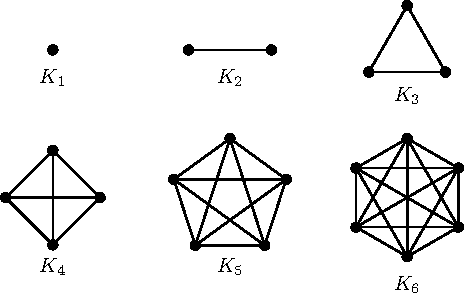
\includegraphics{figures/1_intro_3_complete}
\caption{Grafos completos de ordem 1 até 6.}
\label{fig:intro:complete}
\end{figure}
%%%%%%%%%%%%%%%%%%%%%%%%%%%%%%%%%%%%%%%%

Uma outra família de grafos importante na Teoria de Ramsey é, surpreendentemente, a família dos \indef{grafos vazios}. Um grafo $G$ é vazio quando ele não possui nenhuma aresta. É importante notar que um grafo vazio ainda pode ter vértices.

Uma maneira de relacionar os grafos completos e vazios é por meio da operação de complementação. Seja $G = (V,E)$ um grafo simples. O \indef{complemento} de $G$ é um grafo $\comp{G}$ com o mesmo conjunto de vértices $V$, no qual dois vértices são adjacentes em $\comp{G}$ se e somente se eles não são adjacentes em $G$. Em outras palavras, o conjunto de arestas de $\comp{G}$ é o complemento de $E$ em relação à $V^{(2)}$. Portanto, podemos escrever apenas $\comp{G} = (V,\comp{E})$ e notamos que para todo grafo simples $G$, $\comp{\comp{G}} = G$.
Temos então que o grafo vazio com $n$ vértices é complemento de $K_n$, portanto o denotamos por $\comp{K_n}$.

%%%%%%%%%%%%%%%%%%%%%%%%%%%%%%%%%%%%%%%%
\begin{figure}[ht!]
\centering
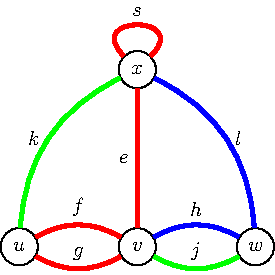
\includegraphics{figures/1_intro_4_excolouring}
\caption{Exemplo de coloração de arestas em três cores.}
\label{fig:intro:excolouring}
\end{figure}
%%%%%%%%%%%%%%%%%%%%%%%%%%%%%%%%%%%%%%%%

Finalmente, o último conceito necessário nesta introdução é o de \indef{coloração de arestas}. A noção de coloração é muito importante em Teoria de Grafos, sendo intimamente relacionada ao surgimento da mesma. A idéia principal de colorações é mapear o conjunto de vértices ou de arestas em um conjunto de cores $\mathcal{C}$. Utiliza-se cores no lugar de índices ou números para enfatizar a ausência de estrutura no conjunto. Assim, se $G = (V,E)$ é um grafo, então uma coloração de arestas de $G$ em $k$ cores é um mapa entre $E$ e um conjunto de $k$ cores, isto é, uma função $c: E(G) \to \mathcal{C}$, no qual $\mathcal{C} = \{ C_1, \dots, C_k\}$ é um conjunto de $k$ cores.
Uma coloração de arestas em $k$ cores também é chamada de $k$-coloração de arestas. Note que se considerarmos apenas arestas de cor $C$ em uma coloração de arestas, temos um subgrafo de $G$, que é denotado por $G_C$.
Neste texto, quando alguma notação incluir $G_C$ como índice, podemos simplificar para apenas $C$. Por exemplo, a vizinhança do vértice $v$ no grafo $G_C$ pode ser denotada por $N_C(v)$ em vez de $N_{G_C}(v)$.

Note também que uma coloração de arestas pode ser vista como uma partição do conjunto de arestas nas partes $c^{-1}(C_i)$. Desta forma, estamos particionando as arestas do grafo em classes determinada pela cor. Por exemplo, a Figura \ref{fig:intro:excolouring} exemplifica uma coloração de arestas em três cores do grafo construído no início desta seção. Esta coloração particiona o conjunto de arestas em $\{k,j\}$, $\{e,f,g,s\}$ e $\{h,l\}$.

%%%%%%%%%%%%%%%%%%%%%%%%%%%%%%%%%%%%%%%%%%%%%%%%%%%%%%%%%%%%%%%%%%%%%%%%%%%%%%%%

\section{Números de Ramsey}

No início do capítulo, vimos o problema das mesas, que nos diz que em mesas de seis alunos, três alunos se conhecem ou três alunos não se conhecem. Consideremos, agora, um grafo $G$ no qual os vértices são os seis alunos na mesa e uma aresta está presente entre dois alunos quando eles se conhecem. Note que $\comp{G}$ é o grafo em que dois alunos são adjacentes quando não se conhecem. O problema das mesas, então, nos diz que se $G$ possui 6 vértices, então $G$ ou $\comp{G}$ possui um triângulo como subgrafo.

Observar o mesmo fato em termos de colorações é ainda mais vantajoso. Novamente, considere $G$ como o grafo em que os vértices são as seis pessoas na festa, mas, desta vez, considere o grafo completo. Realizamos uma coloração das arestas de $G$ em duas cores, $c: E(G) \to \{ R,B \}$ ($R$ e $B$ denotam vermelho e azul, respectivamente), de forma que $c(xy) = R$ se $x$ e $y$ são pessoas que se conheçem e $c(xy) = B$ se $x$ e $y$ são pessoas que não se conhecem. Assim, queremos mostrar que $G$ possui um triângulo monocromático, isto é, um triângulo no qual todas as três arestas tem a mesma cor. Equivalentemente, podemos dizer que $G_R$ ou $G_B$ possuem um triangulo. Considerando esta formalização por colorações de arestas, podemos reformular o Fato \ref{fact:intro:ramsey}.

%%%%%%%%%%%%%%%%%%%%%%%%%%%%%%%%%%%%%%%%
\begin{proposition}
\label{thm:intro:r33}
Se $G$ é um grafo completo com 6 vértices e $c: E(G) \to \{ R,B\}$ é uma coloração de arestas, então $G$ possui um triângulo monocromático.
\end{proposition}
%%%%%%%%%%%%%%%%%%%%%%%%%%%%%%%%%%%%%%%%
\begin{proof}
Seja $v \in V(G)$ um vértice arbitrário e seja $N(v)$ a sua vizinhança. O vértice $v$ se liga aos vértices de $N(v)$ utilizando arestas vermelhas ou azuis. Logo $N(v) = N_R(v) \union N_B(v)$. Como o grau de $v$ é 5, então $d_R(v) + d_B(v) = 5$. Pelo princípio das casas dos pombos, alguma cor dentre $R$ e $B$, digamos $R$, é tal que $d_R(v) >= 3$. Agora, observe que se existem dois vizinhos de $v$ ligados por uma aresta vermelha, então eles formam um triângulo vermelho com $v$. Caso contrário, isto é, não existem dois vizinhos de $v$ ligados por aresta vermelhas, toda aresta com ambas as extremidades em $N_R(v)$ é azul, o que garante que existe um triângulo azul em $v$. Desta forma, em ambos os casos, $G$ possui um triângulo monocromático.
\end{proof}
%%%%%%%%%%%%%%%%%%%%%%%%%%%%%%%%%%%%%%%%

%%%%%%%%%%%%%%%%%%%%%%%%%%%%%%%%%%%%%%%%
\begin{figure}[ht!]
\centering
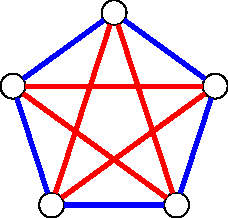
\includegraphics{figures/1_intro_5_pentagram}
\caption{Coloração do $K_5$ sem $K_3$ monocromáticos.}
\label{fig:intro:r33lb}
\end{figure}
%%%%%%%%%%%%%%%%%%%%%%%%%%%%%%%%%%%%%%%%

Algo interessante de notar é que, com 5 vértices, este fato pode ser evitado: existe uma coloração das arestas do $K_5$ que não possúi triângulos monocromáticos, como podemos observar na Figura \ref{fig:intro:r33lb}. Com esta observação, concluímos que 6 é o menor número de vértices que um grafo completo precisa ter de forma que qualquer coloração de suas arestas com duas cores possua um triângulo monocromático.

Agora que entendemos em que condições uma coloração de arestas em duas cores necessariamente possui um triângulo monocromático, podemos estudar quando é possível evitar a existência de outros grafos completos como subgrafo monocromático. Desta forma, é conveniente definir a seguinte quantidade:

%%%%%%%%%%%%%%%%%%%%%%%%%%%%%%%%%%%%%%%%
\begin{definition}
O $k$-ésimo número de Ramsey, $R(k)$, é o menor inteiro positivo $n$ tal que qualquer coloração de arestas em duas cores do grafo $K_n$ possui um $K_k$ monocromático.
\end{definition}
%%%%%%%%%%%%%%%%%%%%%%%%%%%%%%%%%%%%%%%%

Com esta definição, podemos reescrever o enunciado da Proposição \ref{thm:intro:r33} como $R(3) \leq 6$, uma vez que ele nos mostra que 6 vértices são suficientes para encontrar um triângulo monocromático. A observação logo acima em conjunto com a Figura \ref{fig:intro:r33lb} nos indica que $R(3) > 5$. Unindo os dois resultados, obtemos $R(3) = 6$. Este resultado apareceu pela primeira vez como um problema da competição de matemática universitária Putnam\footnote{A William Lowell Putnam Mathematical Competition, comumente referida apenas por Putnam Competition, é uma competição anual de matemática para alunos de graduação no Canada e nos Estados Unidos. No ano de 1953, a segunda questão do primeiro dia enunciava:
\emph{Six points are in general position in space (no three in a line, no four in a plane). The fifteen line segments joining them in pairs are drawn and then painted, some segments red, some blue. Prove that some triangle has all its sides the same color.} \cite{putnam}}, em 1953.

Observamos também que $R(1) = 1$, uma vez que um $K_1$ monocromático é simplesmente um vértice qualquer e que $R(2) = 2$ pois um $K_2$ monocromático é uma aresta qualquer da coloração.

Antes de estudar outros valores conhecidos de $R(k)$ e seguintes generalizações deste conceito, é importante mostrar que eles estão bem-definidos. Ou seja, precisamos verificar que para todo $k$ realmente existe um número $n$ tal que qualquer coloração de arestas do $K_n$ possui um $K_k$ monocromático. Esta questão não é trivial; poderia ser o caso que se $k$ fosse suficientemente grande, fosse possível evitar a existência de $K_k$ monocromáticos em alguma coloração com $n$ arbitrariamente grande. Como vamos ver a seguir, este não é o caso. De fato, vamos encontrar um limitante superior para o número de Ramsey, que é suficiente para determinar que $R(k)$ está bem definido por boa ordem.

%%%%%%%%%%%%%%%%%%%%%%%%%%%%%%%%%%%%%%%%
\begin{theorem}[Ramsey 1930]
\label{thm:intro:ramsey}
Para todo $k \in \mathbb{N}$, $R(k) \leq 2^{2k-2} < 4^k $. Em particular, $R(k)$ está bem definido.
\end{theorem}
%%%%%%%%%%%%%%%%%%%%%%%%%%%%%%%%%%%%%%%%
\begin{proof}
Esta prova consiste em sucessivas aplicações do princípio da casa dos pombos. Seja $G = G^1$ um grafo completo com $n = 2^{l}$ vértices com uma coloração de arestas $c$ em duas cores $R$ e $B$. Vamos encontrar uma cópia monocromática de $K_k$ em $G$ se fizermos $n$ grande o suficiente ao escolher $l$ de forma apropriada.

%%%%%%%%%%%%%%%%%%%%%%%%%%%%%%%%%%%%%%%%
\begin{figure}[ht!]
\centering
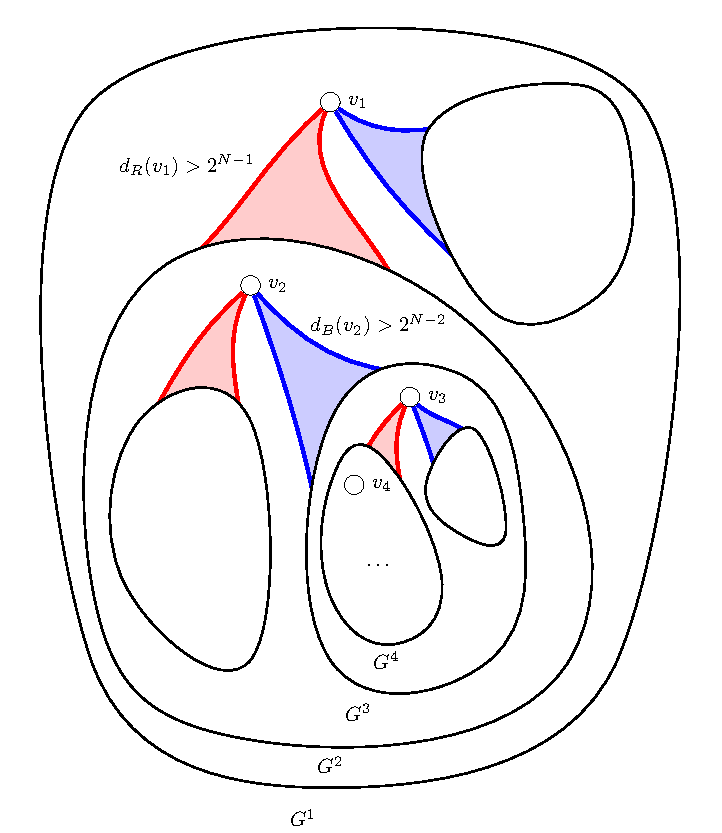
\includegraphics[width=0.7\linewidth]{figures/1_intro_6_recursive}
\caption{Construção recursiva da sequência de vértices $v_i$ e cores.}
\label{fig:intro:recursive}
\end{figure}
%%%%%%%%%%%%%%%%%%%%%%%%%%%%%%%%%%%%%%%%

Seja $v_1 \in V(G^1)$. Por definição, $|N(v_1)| = n-1$. Considere as vizinhanças disjuntas $N_R(v_1)$ e $N_B(v_1)$ e note que $N_R(v_1) \cup N_B(v_1) = N(v_1)$. Pelo Princípio da Casa dos Pombos, ou $|N_R(v_1)| \geq 2^{l-1}$, ou $|N_B(v_1)| \geq 2^{l-1}$.
Note que não é possível que $|N_R(v_1)| < 2^{l-1}$ e $|N_B(v_1)| < 2^{l-1}$ simultaneamente pois $(2^{l-1} - 1) + (2^{l-1} - 1)  = 2^l - 2 < n - 1$.
Denote por $C_1$ a cor que possui a maior vizinhança a partir de $v_1$. Seja $G^2 = G^1[N_{C_1}(v_1)]$, isto é, o subgrafo de $G^1$ induzido pela maior vizinhança de $v_1$. Por construção, $|V(G^2)| \geq 2^{l - 1}$.

Seja $v_2 \in V(G^2)$. Repetindo o raciocínio usado para construir $G^2$, obtemos uma cor $C_2$ e um subgrafo $G^3 = G^2[N_{C_2}(v_2)]$ tal que $|V(G^3)| \geq 2^{l-2}$. Por indução, repetimos este processo e obtemos o subgrafo $G^t$ com $|V(G^j)| \geq 2^{l+1-t}$. Enquanto $2^{l+1-t} \geq 1$, existe alguma vizinhança colorida não vazia, e podemos continuar o processo. Portanto, quando $t = l+1$, garantimos que $G^{l+1}$ possui um vértice, o qual denotamos $v_{l+1}$ e não podemos mais continuar o processo.

Desta forma, obtemos uma sequência de grafos $G^1, G^2, \dots, G^{l+1}$ tal que $|V(G^i)| \geq 2^{l+1-i}$, uma sequência de vértices $v_1, v_2, \dots, v_{l+1}$ com $v_i \in V(G^i)$ e cores $C_1, \dots, C_l$ com a propriedade de que o vértice $v_i$ se conecta a todos os outros vértices seguintes nesta sequência com a cor $C_i$, isto é, $C(v_i v_j) = C_i$ se $j > i$. A Figura \ref{fig:intro:recursive} ilustra este processo.

Finalmente, escolhendo $l = 2k - 2$, obtemos uma sequência de $2k - 1$ vértices e $2k - 2$ cores. Pelo Princípio da Casa dos Pombos, alguma cor aparece pelo menos $k - 1$ vezes, digamos que a cor $C$ ocorre nos índices $C_{a_1} =  C_{a_2} = \dots = C_{a_{k-1}}$. Isto implica que os vértices $v_{a_1}, v_{a_2}, \dots v_{a_{k-1}}$ formam um $K_{k-1}$ monocromático.
No entanto, recorde que o último vértice $v_{l+1}$ recebe arestas de cor $C$ dos vértices $v_{a_{i}}$, portanto, podemos adicioná-lo ao $K_{k-1}$ para obter um $K_k$ monocromático, como queríamos. Com isto, concluímos que $R(k) \leq 2^{2k - 2} < 4^k$.
\end{proof}
%%%%%%%%%%%%%%%%%%%%%%%%%%%%%%%%%%%%%%%%

Embora este teorema seja associado a Frank P. Ramsey, um matemático e filósofo britânico que estudou Lógica, ele não foi provado nesta forma e nem utilizando este método. O teorema na forma como ele provou \cite{ramsey} era sobre conjuntos infinitos, mas a prova original se assemelha em estrutura à prova aqui apresentada.

Agora com o Teorema \ref{thm:intro:ramsey}, sabemos não só que os números de Ramsey estão bem definidos, mas estabelecemos uma cota superior concreta para o seu valor. Nos próximos capítulos, vamos ver generalizações deste resultado, em conjunto com algumas técnicas mais recentes.

%%%%%%%%%%%%%%%%%%%%%%%%%%%%%%%%%%%%%%%%%%%%%%%%%%%%%%%%%%%%%%%%%%%%%%%%%%%%%%%%
